\section{The Raft consensus algorithm}

Raft was proposed by Diego Ongaro and John Ousterhout in 2014. The goal was to offer a easy to understand, implementable and fault-tolerant consensus protocol to be used in a distributed system to replicate state machines. Raft works by managing a replicated log across multiple nodes and upholds simplicity by separating key elements of the process, that is leader election, log distribution and safety, versus a protocol like Paxos that has proven difficult to understand. Key features of Raft include:

\noindent \textbf{Strong leader:} The replication of log entries flow from the leader only. This simplifies log management, and enhances the leader role in Raft compared to other consensus protocols.

\noindent \textbf{Leader election:} From the start of the algorithm a leader has to be elected. Raft uses a randomized timer on each node to elect a leader. This is done to avoid conflicts and assumes all nodes are equally capable of being leaders. The time period electing a leader is called a term, and a new leader must be elected, if the old one fail.

\noindent \textbf{Membership changes:} Raft offers a join and leave command to dynamically change the membership of nodes. This is facilited by what is called a \textit{joint consensus} mechanism, that allows two different configurations to overlap while the transition is ongoing.

\noindent \textbf{Log replication:} The leader is responsible for replicating a log containing state information. During a term, client nodes (followers) send commands to the leader, and these are saved in a log. Upon replication, followers append the entries received from the leader in their own log. When a majority of followers have received the log, a leader adds it to his own state machine and it is then considered committed.

\noindent \textbf{Safety:} Only one leader can be elected for a given term. To ensure consistency, if a server has applied one log entry for an index in its log, then no other server can may apply a different value for the same index. Only a server with the newest log can become leader.

\noindent We will now look at the fundamentals for the protocol. We assume a cluster of five servers ($S_1$ to $S_5$) participating in our Raft consensus algorithm. All nodes have a randomized timer $T_i$ = (i=1,2...,N). Figure \ref{fig:raft} shows the topology and how a majority of the followers have received the log entries for index one to three, hence its committed state. The algorithm works the following way:

\begin{itemize}
	\item 1. The timer of $S_1$ expires first. It starts an election hereby becoming a candidate server, increases the term counter, votes for itself and sends a RPC message to other servers requesting their vote. The current term is included in the message. Servers will vote in  first-come-first-server manner. In case of split votes, Raft simply waits for the timer to timeout, a new term starts and election process repeats.
	\item 2. $S_1$ received the majority of votes, so it has become leader. It keeps in touch with followers by sending out a heartbeat usually every 150 to 300ms. If followers do not receive a heartbeat regularly, they will start a new election.
	\item 3. Now log replication starts. The leader $S_1$ saves requests in its log and marks them with the current term. In figure \ref{fig:raft} the log entries are from term two. The leader must now replicate the log to other servers. Every follower keeps track of the next free index in its log, this position will be assigned the value from the leader. For each follower, the leader keeps track of a match index, that indicate to which index in the log both the leader and the follower agree on the state of the system.
	\item 4. When a majority of followers acknowledge the log entries, they are committed by the leader. For our setup, the majority is three and the minority is two.
\end{itemize}

\noindent Two inconsistency scenarios can occur, so we will quickly cover those: Imagine our leader $S_1$ goes down, and $S_2$ is elected leader. Meanwhile $S_4$ has been down throughout, so its log is empty. When $S_2$ sends out log replications, called RPC AppendEntries, they include a consistency check. If the next index is three (i=3), it includes information about index two (i=i-1). It asks $S_4$ if it has an entry for i=i-1. $S_4$ replies negatively. This continues until $S_4$ has rolled back its next index pointer to the empty log prefix, since it does not include any entries. From here $S_2$ will repair $S_4$'s log by sending AppendEntries to $S_4$ including information for each index.

\noindent Another scenario is extraneous entries. Before $S_1$ went down, it wrote two entries in its own log, but never committed them. As $S_2$ is the new leader, we are now in term two, so entries from term one are no longer valid. If $S_1$ comes back up, $S_2$ will overwrite $S_1$'s old entries with the newer ones, because it is in a newer term. More details on voting and safety are available in the official paper.

\begin{figure}[H]
	\centering
	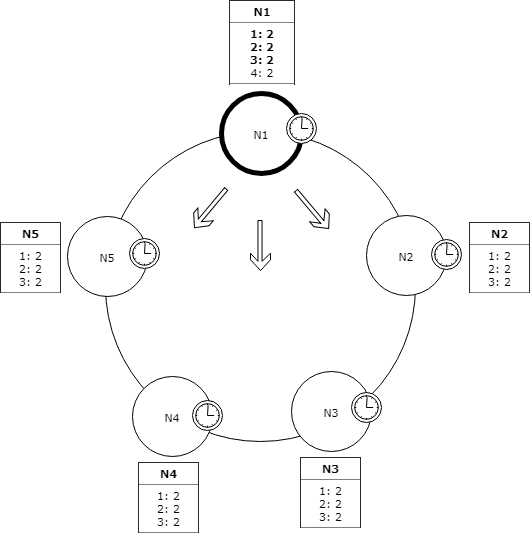
\includegraphics[scale=0.4]{faultTolerance/fig/Raft.png}
	\caption{The topology for our Raft setup. N1 is leader and replicates its state log to follower nodes.}
	\label{fig:raft}
\end{figure}


